
%----------------------------------------------------------------------------------------
%	Lecture 28
%----------------------------------------------------------------------------------------

\chapter{Stokes' Theorem Continued} 

\bigbreak

\section{Conservative Fields in Space}

{\bf Theorem : } If a vector field {\bf F} is defined and differentiable in a simply connected region
and $\nabla \times {\bf F} = 0$ everywhere in the region then ${\bf F}$ is a gradient field.
And the line integral of ${\bf F}$ is path independent.

We can prove this using the same methods as the Green's Theorem.
The only difference will be that instead of taking the plane we will have to find a surface whose boundary is our curve.
This is where  simply connected region comes in. 
We can always find such a surface because the region is simply connected.


\section{Orientability}

A mobius strip in space is a surface which has only one side,
and if you try to orient it using then you will reach a contradiction.

\begin{figure}[ht!]
    \centering
    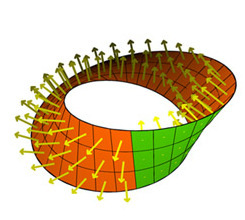
\includegraphics[scale=0.5]{./images/lecture_28_figure_1.png}
    \caption{Mobius Strip with Normal Vectors}
\end{figure}

Here we can see that as we go along the mobius strip the normal vector changes directions.

So that is why we call it a non-orientable surface.

Since it has only one side so we cannot speak about flux.
So flux cannot be defined.

\section{Stokes' Theorem and Surface Independent}

Let's say we have a curve $C$ in space and two surfaces $S_1$ and $S_2$.

\begin{figure}[ht!]
    \centering
    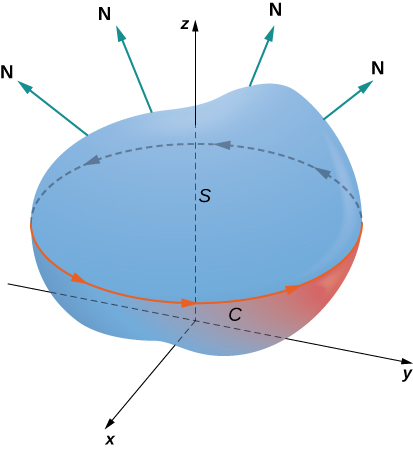
\includegraphics[scale=0.7]{./images/lecture_28_figure_2.jpg}
    \caption{Surface Independence}
\end{figure}

Here, the normal vector for $S_1$ and $S_2$ will both be upwards.
So by Stokes' Theorem, we have,
$$ \oint_C {\bf F} d{\bf r} = \iint_{S_1} \nabla \times {\bf F} dA = \iint_{S_2} \nabla \times {\bf F} dA $$

By subtracting, we get 
$$ \iint_{S_1} \nabla \times {\bf F} dA - \iint_{S_2} \nabla \times {\bf F} dA = \iint_{S} \nabla \times {\bf F} dA $$

Here, $S$ is $S_1$ and $S_2$ combined with normal vector pointing outwards as subtracting is the same as inverting the normal vector.

Now this is the flux of a function through a closed surface $S$ which encloses a region $D$.
So by Divergence Theorem,

$$ \iint_S \nabla \times {\bf F} dA = \iiint_D \nabla \cdot (\nabla \times {\bf F}) dV $$

We can prove that the divergence of a curl is always zero.

\begin{align*}
div( curl({\bf F}) ) 
    & = div(\ijk{(R_y - Q_z)}{(R_x - P_z)}{(P_y - Q_x)}) \\
    & = R_{yx} - Q_{zx} + R_{xy} - P_{zy} + P_{yz} - Q_{xz} \\
div( curl( {\bf F} )) & = \nabla \cdot (\nabla \times {\bf F}) = 0
\end{align*} 

{\bf Note : } For any two vectors ${\bf u}$ and  ${\bf v}$, ${\bf u} \cdot ({\bf u} \times {\bf v}) = 0$ 
because $({\bf u} \times {\bf v})$ is perpendicular to ${\bf u}$ and ${\bf v}$ both.
So even though $\nabla$ is not a real vector, but sometimes we can treat it as such.

